% Options for packages loaded elsewhere
\PassOptionsToPackage{unicode}{hyperref}
\PassOptionsToPackage{hyphens}{url}
%
\documentclass[
]{article}
\usepackage{amsmath,amssymb}
\usepackage{lmodern}
\usepackage{iftex}
\ifPDFTeX
  \usepackage[T1]{fontenc}
  \usepackage[utf8]{inputenc}
  \usepackage{textcomp} % provide euro and other symbols
\else % if luatex or xetex
  \usepackage{unicode-math}
  \defaultfontfeatures{Scale=MatchLowercase}
  \defaultfontfeatures[\rmfamily]{Ligatures=TeX,Scale=1}
\fi
% Use upquote if available, for straight quotes in verbatim environments
\IfFileExists{upquote.sty}{\usepackage{upquote}}{}
\IfFileExists{microtype.sty}{% use microtype if available
  \usepackage[]{microtype}
  \UseMicrotypeSet[protrusion]{basicmath} % disable protrusion for tt fonts
}{}
\makeatletter
\@ifundefined{KOMAClassName}{% if non-KOMA class
  \IfFileExists{parskip.sty}{%
    \usepackage{parskip}
  }{% else
    \setlength{\parindent}{0pt}
    \setlength{\parskip}{6pt plus 2pt minus 1pt}}
}{% if KOMA class
  \KOMAoptions{parskip=half}}
\makeatother
\usepackage{xcolor}
\usepackage[margin=1in]{geometry}
\usepackage{color}
\usepackage{fancyvrb}
\newcommand{\VerbBar}{|}
\newcommand{\VERB}{\Verb[commandchars=\\\{\}]}
\DefineVerbatimEnvironment{Highlighting}{Verbatim}{commandchars=\\\{\}}
% Add ',fontsize=\small' for more characters per line
\usepackage{framed}
\definecolor{shadecolor}{RGB}{248,248,248}
\newenvironment{Shaded}{\begin{snugshade}}{\end{snugshade}}
\newcommand{\AlertTok}[1]{\textcolor[rgb]{0.94,0.16,0.16}{#1}}
\newcommand{\AnnotationTok}[1]{\textcolor[rgb]{0.56,0.35,0.01}{\textbf{\textit{#1}}}}
\newcommand{\AttributeTok}[1]{\textcolor[rgb]{0.77,0.63,0.00}{#1}}
\newcommand{\BaseNTok}[1]{\textcolor[rgb]{0.00,0.00,0.81}{#1}}
\newcommand{\BuiltInTok}[1]{#1}
\newcommand{\CharTok}[1]{\textcolor[rgb]{0.31,0.60,0.02}{#1}}
\newcommand{\CommentTok}[1]{\textcolor[rgb]{0.56,0.35,0.01}{\textit{#1}}}
\newcommand{\CommentVarTok}[1]{\textcolor[rgb]{0.56,0.35,0.01}{\textbf{\textit{#1}}}}
\newcommand{\ConstantTok}[1]{\textcolor[rgb]{0.00,0.00,0.00}{#1}}
\newcommand{\ControlFlowTok}[1]{\textcolor[rgb]{0.13,0.29,0.53}{\textbf{#1}}}
\newcommand{\DataTypeTok}[1]{\textcolor[rgb]{0.13,0.29,0.53}{#1}}
\newcommand{\DecValTok}[1]{\textcolor[rgb]{0.00,0.00,0.81}{#1}}
\newcommand{\DocumentationTok}[1]{\textcolor[rgb]{0.56,0.35,0.01}{\textbf{\textit{#1}}}}
\newcommand{\ErrorTok}[1]{\textcolor[rgb]{0.64,0.00,0.00}{\textbf{#1}}}
\newcommand{\ExtensionTok}[1]{#1}
\newcommand{\FloatTok}[1]{\textcolor[rgb]{0.00,0.00,0.81}{#1}}
\newcommand{\FunctionTok}[1]{\textcolor[rgb]{0.00,0.00,0.00}{#1}}
\newcommand{\ImportTok}[1]{#1}
\newcommand{\InformationTok}[1]{\textcolor[rgb]{0.56,0.35,0.01}{\textbf{\textit{#1}}}}
\newcommand{\KeywordTok}[1]{\textcolor[rgb]{0.13,0.29,0.53}{\textbf{#1}}}
\newcommand{\NormalTok}[1]{#1}
\newcommand{\OperatorTok}[1]{\textcolor[rgb]{0.81,0.36,0.00}{\textbf{#1}}}
\newcommand{\OtherTok}[1]{\textcolor[rgb]{0.56,0.35,0.01}{#1}}
\newcommand{\PreprocessorTok}[1]{\textcolor[rgb]{0.56,0.35,0.01}{\textit{#1}}}
\newcommand{\RegionMarkerTok}[1]{#1}
\newcommand{\SpecialCharTok}[1]{\textcolor[rgb]{0.00,0.00,0.00}{#1}}
\newcommand{\SpecialStringTok}[1]{\textcolor[rgb]{0.31,0.60,0.02}{#1}}
\newcommand{\StringTok}[1]{\textcolor[rgb]{0.31,0.60,0.02}{#1}}
\newcommand{\VariableTok}[1]{\textcolor[rgb]{0.00,0.00,0.00}{#1}}
\newcommand{\VerbatimStringTok}[1]{\textcolor[rgb]{0.31,0.60,0.02}{#1}}
\newcommand{\WarningTok}[1]{\textcolor[rgb]{0.56,0.35,0.01}{\textbf{\textit{#1}}}}
\usepackage{graphicx}
\makeatletter
\def\maxwidth{\ifdim\Gin@nat@width>\linewidth\linewidth\else\Gin@nat@width\fi}
\def\maxheight{\ifdim\Gin@nat@height>\textheight\textheight\else\Gin@nat@height\fi}
\makeatother
% Scale images if necessary, so that they will not overflow the page
% margins by default, and it is still possible to overwrite the defaults
% using explicit options in \includegraphics[width, height, ...]{}
\setkeys{Gin}{width=\maxwidth,height=\maxheight,keepaspectratio}
% Set default figure placement to htbp
\makeatletter
\def\fps@figure{htbp}
\makeatother
\setlength{\emergencystretch}{3em} % prevent overfull lines
\providecommand{\tightlist}{%
  \setlength{\itemsep}{0pt}\setlength{\parskip}{0pt}}
\setcounter{secnumdepth}{-\maxdimen} % remove section numbering
\ifLuaTeX
  \usepackage{selnolig}  % disable illegal ligatures
\fi
\IfFileExists{bookmark.sty}{\usepackage{bookmark}}{\usepackage{hyperref}}
\IfFileExists{xurl.sty}{\usepackage{xurl}}{} % add URL line breaks if available
\urlstyle{same} % disable monospaced font for URLs
\hypersetup{
  pdftitle={HW 3 - Beimnet Taye},
  hidelinks,
  pdfcreator={LaTeX via pandoc}}

\title{HW 3 - Beimnet Taye}
\author{}
\date{\vspace{-2.5em}2023-02-13}

\begin{document}
\maketitle

\hypertarget{p1}{%
\subsection{P1}\label{p1}}

\hypertarget{section}{%
\subsubsection{1}\label{section}}

\begin{itemize}
\tightlist
\item
  Distributions allow us to better visualize the probability of certain
  events that random variables assign. CDFs, PDFs, and quantile
  functions all allow us to directly quantify probabilities of events
  without us having to get the pre-image of the RV's output to derive
  the same information.
\end{itemize}

\hypertarget{p2}{%
\subsection{P2}\label{p2}}

\hypertarget{section-1}{%
\subsubsection{1}\label{section-1}}

\begin{Shaded}
\begin{Highlighting}[]
  \CommentTok{\# TALBE}
\NormalTok{    values }\OtherTok{\textless{}{-}} \FunctionTok{tibble}\NormalTok{(}\AttributeTok{w =} \FunctionTok{seq}\NormalTok{(}\DecValTok{0}\NormalTok{,}\DecValTok{1}\NormalTok{,}\AttributeTok{length =} \DecValTok{1000}\NormalTok{),}
                     \AttributeTok{X =}\NormalTok{ w}\SpecialCharTok{\^{}}\DecValTok{2}\NormalTok{,}
                     \AttributeTok{Y =}\NormalTok{ (}\DecValTok{1}\SpecialCharTok{{-}}\NormalTok{w)}\SpecialCharTok{\^{}}\DecValTok{2}\NormalTok{,)}
    
  \CommentTok{\# CDF FUNCTION}
\NormalTok{    CDF }\OtherTok{\textless{}{-}} \ControlFlowTok{function}\NormalTok{(df, rv) \{}
      
\NormalTok{      rv }\OtherTok{\textless{}{-}} \FunctionTok{enquo}\NormalTok{(rv)}
\NormalTok{      df }\SpecialCharTok{\%\textgreater{}\%} 
        \FunctionTok{arrange}\NormalTok{(}\SpecialCharTok{!!}\NormalTok{rv) }\SpecialCharTok{\%\textgreater{}\%} 
        \FunctionTok{mutate}\NormalTok{(}\AttributeTok{p =} \FunctionTok{row\_number}\NormalTok{()}\SpecialCharTok{/}\FunctionTok{nrow}\NormalTok{(df)) }\SpecialCharTok{\%\textgreater{}\%} 
        \FunctionTok{ggplot}\NormalTok{() }\SpecialCharTok{+}
        \FunctionTok{geom\_line}\NormalTok{(}\FunctionTok{aes}\NormalTok{(}\AttributeTok{x =} \SpecialCharTok{!!}\NormalTok{rv, }\AttributeTok{y =}\NormalTok{ p)) }
      
\NormalTok{    \}}
  \CommentTok{\# X CDF}
\NormalTok{    X\_CDF }\OtherTok{\textless{}{-}} \FunctionTok{CDF}\NormalTok{(values,X)}
\NormalTok{    X\_CDF}
\end{Highlighting}
\end{Shaded}

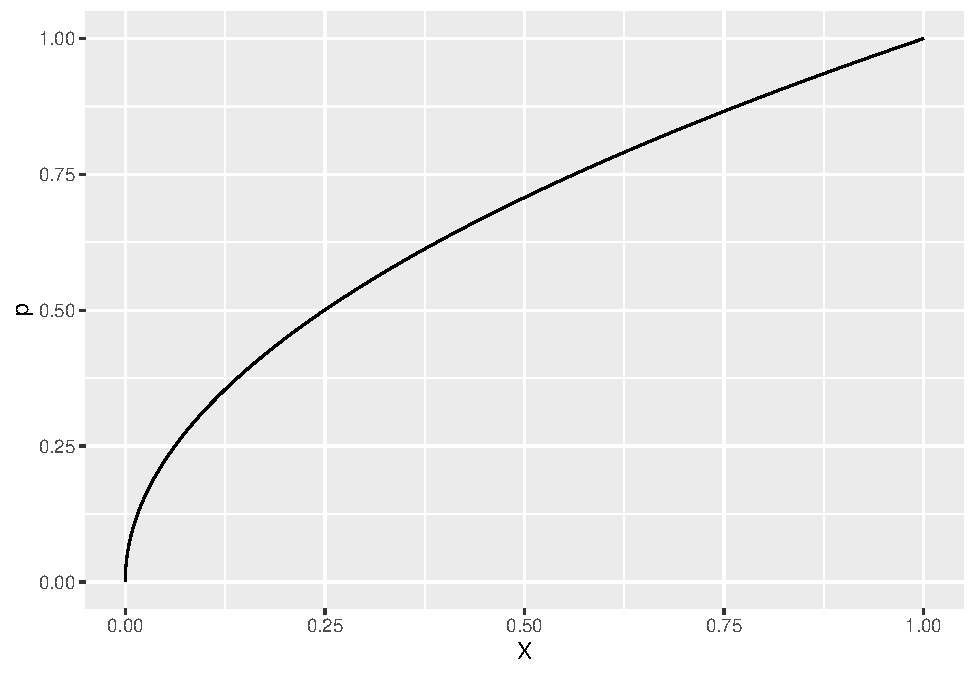
\includegraphics{HW-3_files/figure-latex/unnamed-chunk-1-1.pdf}

\begin{Shaded}
\begin{Highlighting}[]
  \CommentTok{\# X PDF}
\NormalTok{    X\_PDF }\OtherTok{\textless{}{-}}\NormalTok{ values }\SpecialCharTok{\%\textgreater{}\%} 
      \FunctionTok{ggplot}\NormalTok{()}\SpecialCharTok{+}
      \FunctionTok{geom\_histogram}\NormalTok{(}\FunctionTok{aes}\NormalTok{(}\AttributeTok{x =}\NormalTok{ X), }\AttributeTok{binwidth =}\NormalTok{ .}\DecValTok{01}\NormalTok{)}
    
\NormalTok{    X\_PDF}
\end{Highlighting}
\end{Shaded}

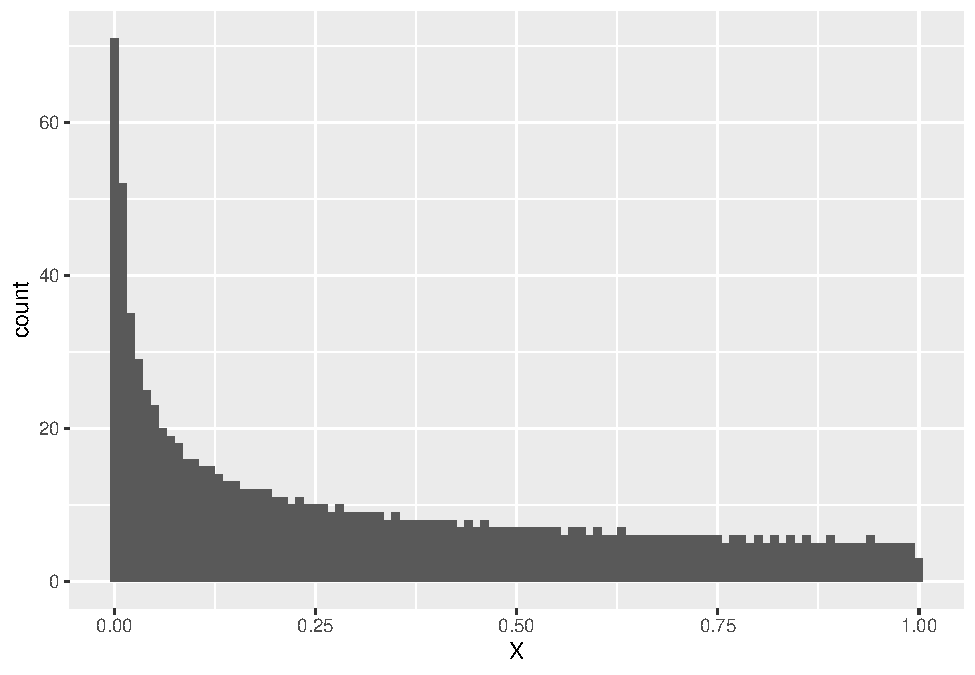
\includegraphics{HW-3_files/figure-latex/unnamed-chunk-1-2.pdf}

\begin{Shaded}
\begin{Highlighting}[]
  \CommentTok{\# Y CDF}
\NormalTok{Y\_CDF }\OtherTok{\textless{}{-}} \FunctionTok{CDF}\NormalTok{(}\AttributeTok{df=}\NormalTok{values,}\AttributeTok{rv =}\NormalTok{ Y)}

\NormalTok{Y\_CDF}
\end{Highlighting}
\end{Shaded}

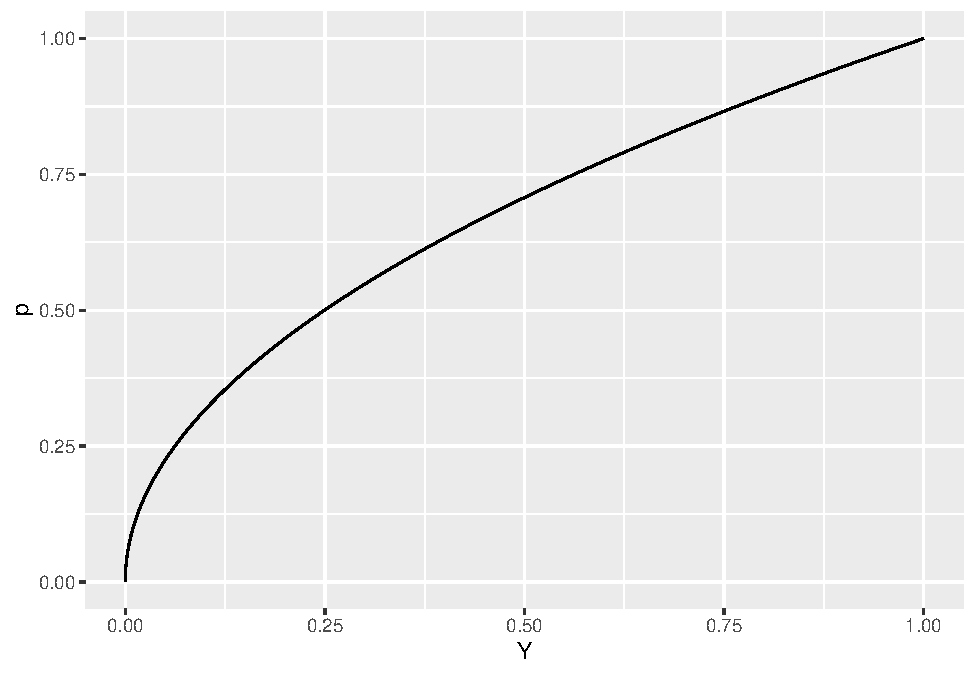
\includegraphics{HW-3_files/figure-latex/unnamed-chunk-1-3.pdf}

\begin{Shaded}
\begin{Highlighting}[]
  \CommentTok{\# Y PDF}

\NormalTok{Y\_PDF }\OtherTok{\textless{}{-}}\NormalTok{ values }\SpecialCharTok{\%\textgreater{}\%} 
  \FunctionTok{ggplot}\NormalTok{()}\SpecialCharTok{+}
  \FunctionTok{geom\_histogram}\NormalTok{(}\FunctionTok{aes}\NormalTok{(}\AttributeTok{x =}\NormalTok{ Y), }\AttributeTok{binwidth =}\NormalTok{ .}\DecValTok{01}\NormalTok{)}

\NormalTok{Y\_PDF}
\end{Highlighting}
\end{Shaded}

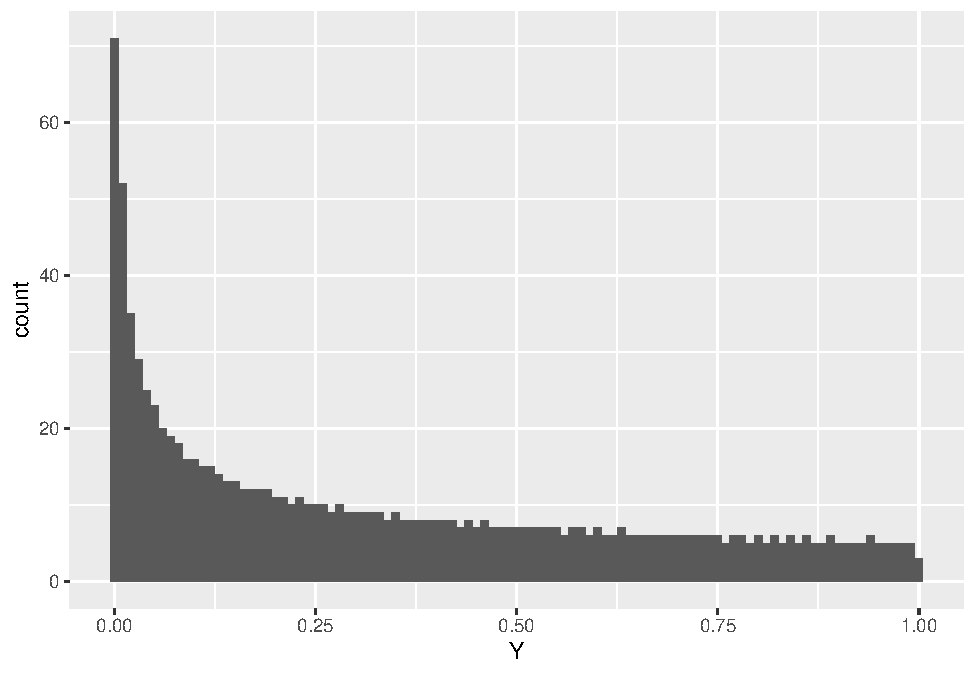
\includegraphics{HW-3_files/figure-latex/unnamed-chunk-1-4.pdf}

\hypertarget{section-2}{%
\subsubsection{2 \& 3}\label{section-2}}

\begin{Shaded}
\begin{Highlighting}[]
\CommentTok{\#TABLE}
\NormalTok{custom }\OtherTok{\textless{}{-}} \FunctionTok{tibble}\NormalTok{(}\AttributeTok{w =} \FunctionTok{seq}\NormalTok{(}\DecValTok{0}\NormalTok{,}\DecValTok{1}\NormalTok{,}\AttributeTok{length =} \DecValTok{1000}\NormalTok{),}
                 \AttributeTok{X =} \DecValTok{2}\SpecialCharTok{\^{}}\NormalTok{w,}
                 \AttributeTok{Y =} \DecValTok{2}\SpecialCharTok{\^{}}\NormalTok{(}\DecValTok{1}\SpecialCharTok{{-}}\NormalTok{w))}
\CommentTok{\# CUSTOM X CDF}
\NormalTok{CX\_CDF }\OtherTok{\textless{}{-}} \FunctionTok{CDF}\NormalTok{(custom,X)}

\NormalTok{CX\_CDF}
\end{Highlighting}
\end{Shaded}

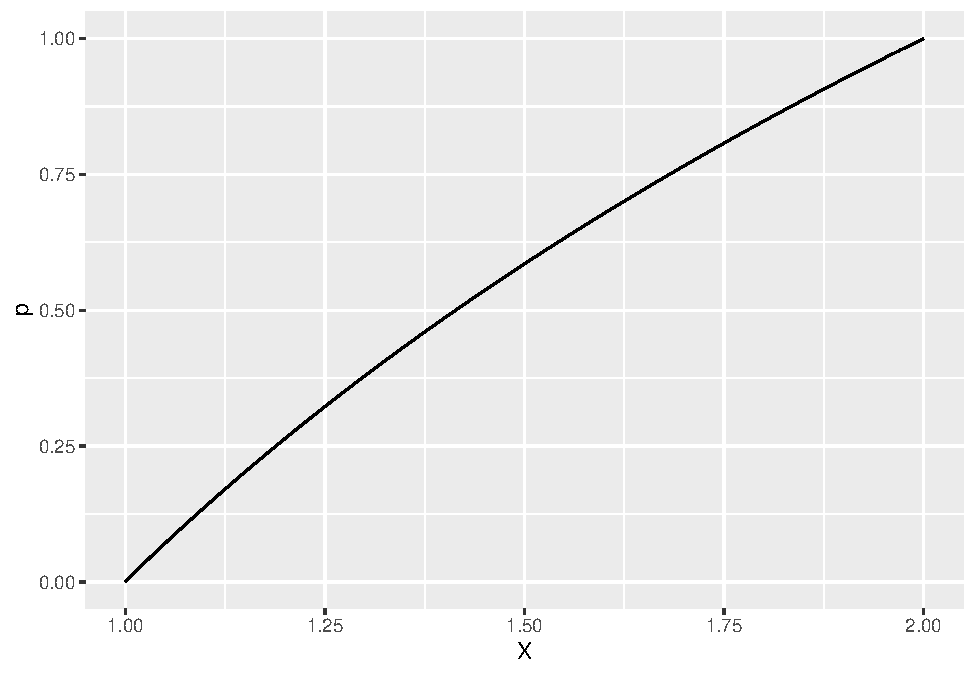
\includegraphics{HW-3_files/figure-latex/unnamed-chunk-2-1.pdf}

\begin{Shaded}
\begin{Highlighting}[]
\CommentTok{\# CUSTOM X PDF}

\NormalTok{CX\_PDF }\OtherTok{\textless{}{-}}\NormalTok{ custom }\SpecialCharTok{\%\textgreater{}\%} 
  \FunctionTok{ggplot}\NormalTok{()}\SpecialCharTok{+}
  \FunctionTok{geom\_histogram}\NormalTok{(}\FunctionTok{aes}\NormalTok{(}\AttributeTok{x =}\NormalTok{ X))}

\NormalTok{CX\_PDF}
\end{Highlighting}
\end{Shaded}

\begin{verbatim}
## `stat_bin()` using `bins = 30`. Pick better value with `binwidth`.
\end{verbatim}

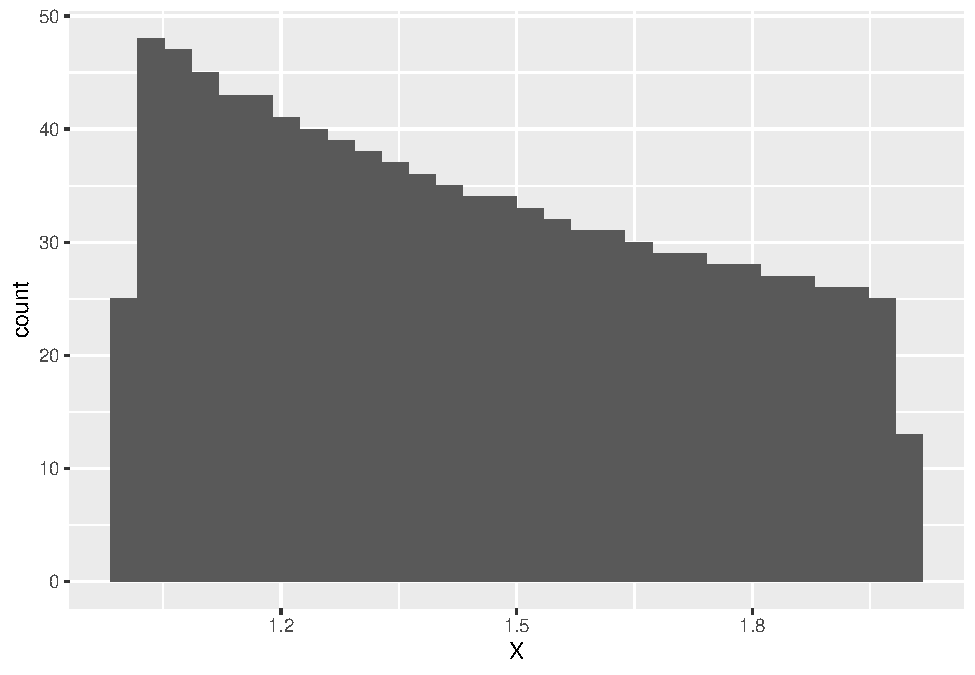
\includegraphics{HW-3_files/figure-latex/unnamed-chunk-2-2.pdf}

\begin{Shaded}
\begin{Highlighting}[]
\CommentTok{\# CUSTOM Y CDF}
\NormalTok{CY\_CDF }\OtherTok{\textless{}{-}} \FunctionTok{CDF}\NormalTok{(custom,Y)}

\NormalTok{CY\_CDF}
\end{Highlighting}
\end{Shaded}

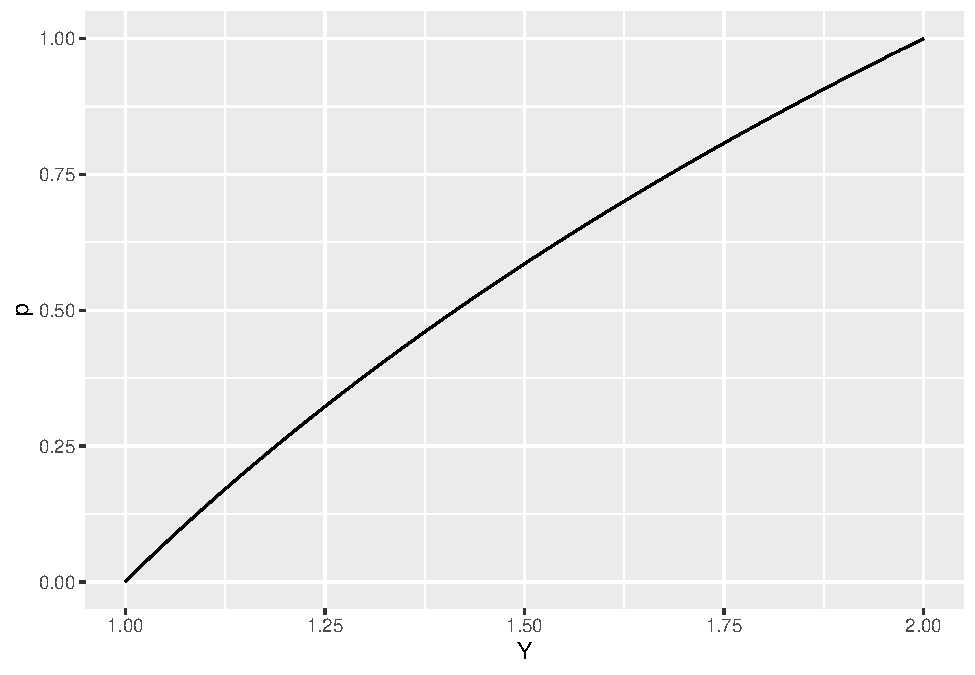
\includegraphics{HW-3_files/figure-latex/unnamed-chunk-2-3.pdf}

\begin{Shaded}
\begin{Highlighting}[]
\CommentTok{\# CUSTOM Y PDF}
\NormalTok{CY\_PDF }\OtherTok{\textless{}{-}}\NormalTok{ custom }\SpecialCharTok{\%\textgreater{}\%} 
  \FunctionTok{ggplot}\NormalTok{()}\SpecialCharTok{+}
  \FunctionTok{geom\_histogram}\NormalTok{(}\FunctionTok{aes}\NormalTok{(}\AttributeTok{x =}\NormalTok{ Y))}

\NormalTok{CY\_PDF}
\end{Highlighting}
\end{Shaded}

\begin{verbatim}
## `stat_bin()` using `bins = 30`. Pick better value with `binwidth`.
\end{verbatim}

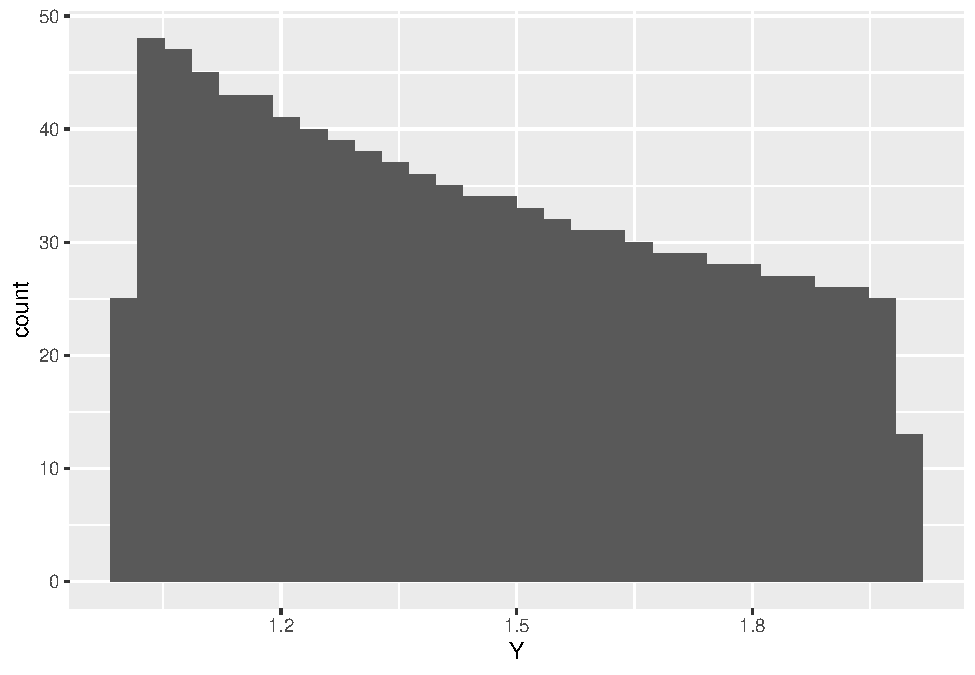
\includegraphics{HW-3_files/figure-latex/unnamed-chunk-2-4.pdf}

\hypertarget{p3}{%
\subsection{P3}\label{p3}}

\hypertarget{section-3}{%
\subsubsection{1}\label{section-3}}

\begin{Shaded}
\begin{Highlighting}[]
\CommentTok{\# quantile function}
\NormalTok{qlap }\OtherTok{\textless{}{-}} \ControlFlowTok{function}\NormalTok{(p, }\AttributeTok{a =} \DecValTok{0}\NormalTok{, }\AttributeTok{b =} \DecValTok{1}\NormalTok{) \{}
  \FunctionTok{return}\NormalTok{(}\FunctionTok{case\_when}\NormalTok{(}\DecValTok{0} \SpecialCharTok{\textless{}=}\NormalTok{ p }\SpecialCharTok{\&}\NormalTok{ p }\SpecialCharTok{\textless{}} \FloatTok{0.5} \SpecialCharTok{\textasciitilde{}}\NormalTok{ a}\SpecialCharTok{+}\NormalTok{b}\SpecialCharTok{*}\FunctionTok{log}\NormalTok{(}\DecValTok{2}\SpecialCharTok{*}\NormalTok{p),}
\NormalTok{            p }\SpecialCharTok{\textgreater{}=} \FloatTok{0.5} \SpecialCharTok{\&}\NormalTok{ p }\SpecialCharTok{\textless{}=} \DecValTok{1} \SpecialCharTok{\textasciitilde{}}\NormalTok{ a}\SpecialCharTok{{-}}\NormalTok{b}\SpecialCharTok{*}\FunctionTok{log}\NormalTok{(}\DecValTok{2}\SpecialCharTok{*}\NormalTok{(}\DecValTok{1}\SpecialCharTok{{-}}\NormalTok{p)),}
\NormalTok{        )}
\NormalTok{  )}
\NormalTok{\}}
\CommentTok{\# Sampling function}
\NormalTok{rlaplace }\OtherTok{\textless{}{-}} \ControlFlowTok{function}\NormalTok{(n,}\AttributeTok{location =} \DecValTok{0}\NormalTok{,}\AttributeTok{scale =} \DecValTok{1}\NormalTok{) \{}
  \FunctionTok{tibble}\NormalTok{(}\AttributeTok{p =} \FunctionTok{runif}\NormalTok{(n),}
         \AttributeTok{X =} \FunctionTok{qlap}\NormalTok{(p,location,scale)) }\SpecialCharTok{\%\textgreater{}\%} 
    \FunctionTok{pull}\NormalTok{(X)}
\NormalTok{\}}
\end{Highlighting}
\end{Shaded}

\hypertarget{section-4}{%
\subsubsection{2}\label{section-4}}

\begin{Shaded}
\begin{Highlighting}[]
\NormalTok{lap\_PDF }\OtherTok{\textless{}{-}} \FunctionTok{ggplot}\NormalTok{() }\SpecialCharTok{+}
  \FunctionTok{geom\_histogram}\NormalTok{(}\FunctionTok{aes}\NormalTok{(}\AttributeTok{x =} \FunctionTok{rlaplace}\NormalTok{(}\DecValTok{10000}\NormalTok{)))}
\NormalTok{lap\_PDF}
\end{Highlighting}
\end{Shaded}

\begin{verbatim}
## `stat_bin()` using `bins = 30`. Pick better value with `binwidth`.
\end{verbatim}

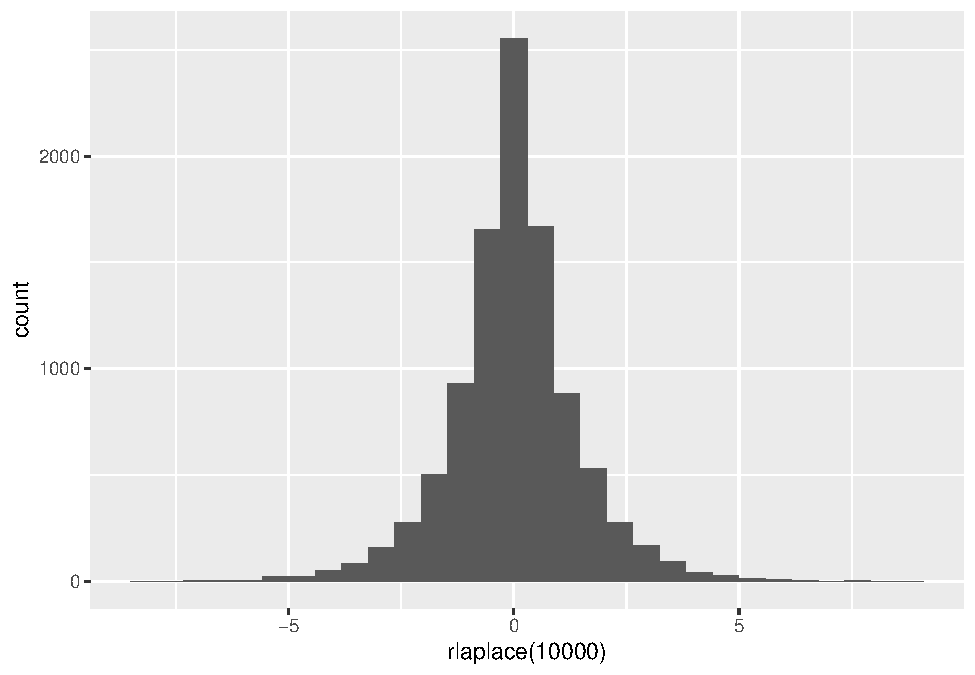
\includegraphics{HW-3_files/figure-latex/unnamed-chunk-4-1.pdf}

\begin{Shaded}
\begin{Highlighting}[]
\NormalTok{lap\_CDF }\OtherTok{\textless{}{-}} \FunctionTok{tibble}\NormalTok{(}\AttributeTok{p =} \FunctionTok{seq}\NormalTok{(}\DecValTok{0}\NormalTok{,}\DecValTok{1}\NormalTok{,}\AttributeTok{length =} \DecValTok{1000}\NormalTok{),}
              \AttributeTok{X =} \FunctionTok{qlap}\NormalTok{(p)) }\SpecialCharTok{\%\textgreater{}\%} 
  \FunctionTok{ggplot}\NormalTok{() }\SpecialCharTok{+}
  \FunctionTok{geom\_line}\NormalTok{(}\FunctionTok{aes}\NormalTok{(}\AttributeTok{x =}\NormalTok{ X, }\AttributeTok{y =}\NormalTok{ p))}
\NormalTok{lap\_CDF}
\end{Highlighting}
\end{Shaded}

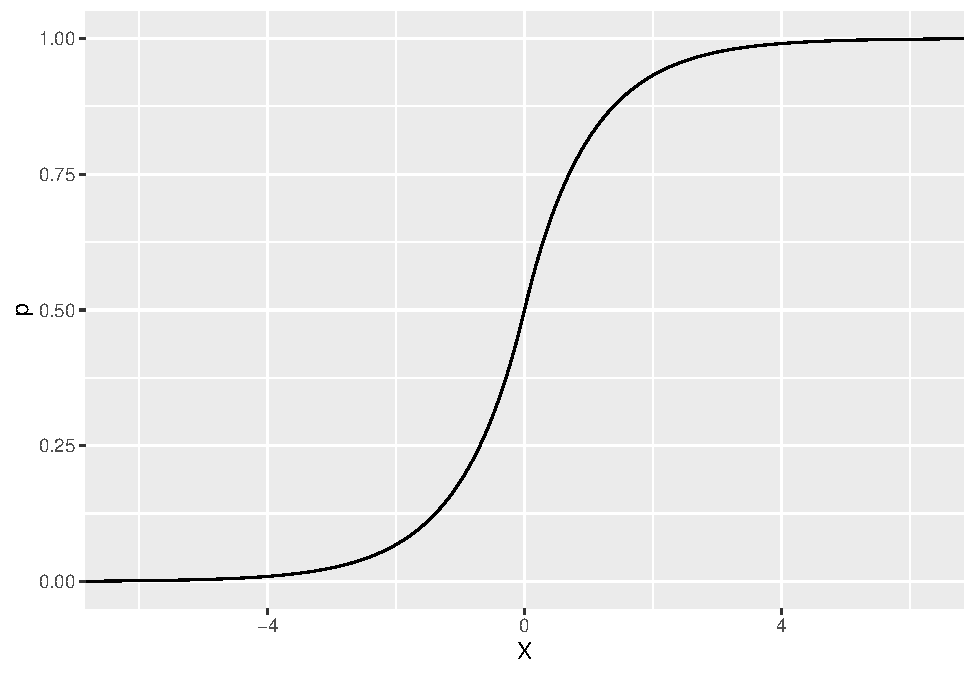
\includegraphics{HW-3_files/figure-latex/unnamed-chunk-4-2.pdf}

\hypertarget{p4}{%
\subsection{P4}\label{p4}}

\hypertarget{section-5}{%
\subsubsection{1}\label{section-5}}

\begin{itemize}
\tightlist
\item
  \(P(Y>-102) = \frac{1}{3}\)
\end{itemize}

\hypertarget{section-6}{%
\subsubsection{2}\label{section-6}}

\begin{itemize}
\tightlist
\item
  \(P(0.5<X<1) = 0.95 - 0.25 = 0.7\)
\end{itemize}

\hypertarget{p5}{%
\subsection{P5}\label{p5}}

\hypertarget{section-7}{%
\subsubsection{1}\label{section-7}}

\begin{itemize}
\tightlist
\item
  Height in a given population is probably normally distributed as
  individual height will symmetrically cluster around the population
  mean and symmetrically taper off in frequency on both sides as the
  height measures get more extreme.
\end{itemize}

\hypertarget{section-8}{%
\subsubsection{2}\label{section-8}}

\begin{itemize}
\tightlist
\item
  A fair coin toss has a Bernoulli distribution as it is a discrete
  distribution with two possible outcomes: heads or tails, with a
  probability of 0.5 for either outcome.
\end{itemize}

\hypertarget{section-9}{%
\subsubsection{3}\label{section-9}}

\begin{itemize}
\tightlist
\item
  The number of work place accidents at a construction site in a year
  probably has a poisson distribution. The number of workplace accidents
  is a countable event within a given time interval, is relatively rare,
  and the probability of the occurrence of one accident is independent
  of the probability of the occurrence of another.
\end{itemize}

\hypertarget{section-10}{%
\subsubsection{4}\label{section-10}}

\begin{itemize}
\tightlist
\item
  The probability of rolling a particular value on a six sided die is
  uniformly distributed as each value has an equal probability of
  occurrence (1/6).
\end{itemize}

\hypertarget{section-11}{%
\subsubsection{5}\label{section-11}}

\begin{itemize}
\tightlist
\item
  The amount of time it takes to receive an order of chicken nuggets
  from a particular McDonalds location is probably exponentially
  distributed as the wait times will cluster around relatively small
  values (it's just chicken nuggets) and dramatically fall off from
  there in an exponential fashion.
\end{itemize}

\end{document}
